\chapter{Metodologia}
\label{cap:metodologia}
 Este capítulo descreve a nossa proposta de visualização para exploração dos
fluxos no tráfego de veículos. O objetivo principal da visualização é centrado
nas propriedades espaciais e temporais dos dados para entender como são os
fluxos de origem e destino pela cidade ao longo do tempo. Buscamos um maior
nível de detalhes através de uma abordagem multinível para explorar padrões
globais e locais do tráfego, com diferentes níveis de agregação temporais e
espaciais.

 Apresentamos inicialmente a ferramenta que estamos desenvolvendo dentro da
nossa proposta, dando uma visão geral dos seus componentes e dos artefatos de
entrada e saída que irão resultar na visualização e análise dos dados. A
ferramenta faz parte do ecossistema de soluções para cidades inteligentes que
são desenvolvidas no contexto do projeto InterSCity\footnote{\rurl{interscity.org}}. Em seguida detalhamos os
conjuntos de dados que iremos utilizar e suas características, e por fim,
explicamos as técnicas que pretendemos aplicar para destacar as propriedades
dos dados dentro da visualização.

\section{Implementação da Visualização}
  Apenas alguns poucos algoritmos de \emph{bundling} são implementados em
bibliotecas de uso aberto. A maioria dos trabalhos pesquisados não apontam
a fonte para as suas ferramentas e implementação dos seus algoritmos. Optamos
então por partir de uma implementação própria para a visualização dos dados,
apoiando-nos em bibliotecas já existentes para exploração de dados geoespaciais.

  Apresentamos então, o InterSCityPlotter, uma ferramenta para análise de dados
do tráfego que permite a criação de múltiplas visualizações, como visualizações
estáticas, ilustrado na Figura \ref{fig:simulated-traffic}, visualizações
baseadas em pontos pontos, ilustrado na Figura \ref{fig:rastro}. Idealizamos a
ferramenta com o objetivo de suportar estudos com dados do trânsito gerados
pelo InterSCSimulator e também por outras fontes, com o propósito de abranger
análises de dados geoespaciais de modo geral, tão importantes no planejamento
das cidades. O diagrama da Figura \ref{fig:interscityplotter} mostra uma visão
geral dos componentes da ferramenta os quais damos uma breve descrição em
seguida.

\begin{figure}[!htb]
  \centering
  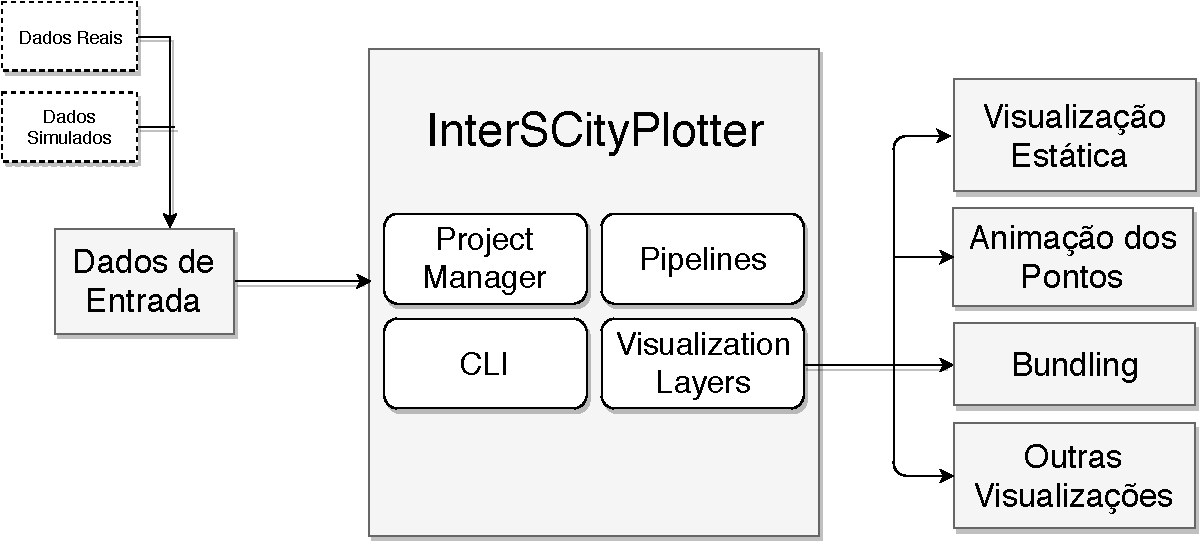
\includegraphics[width=1\textwidth]{../figuras/interscityplotter.pdf}
  \caption{Visão geral da arquitetura da ferramenta InterSCityPlotter que permite a criação
de múltiplas visualizações de dados geoespaciais.}
  \label{fig:interscityplotter}
\end{figure}

\begin{description}
  \item[\emph{ProjectManager}:] A exploração de dados do tráfego começa com a criação de um
novo projeto de visualização a partir de um conjunto de dados de entrada. Esse
componente é responsável pela criação, exclusão e outras ações de gerenciamento
dos projetos. Para utilizar a ferramenta, é necessário criar um novo projeto
apontando o conjunto de dados em um formato CSV. Os dados irão passar por algumas
etapas de pré-processamento definidos no componente \emph{Pipelines} para que
estejam prontos para visualização junto com os arquivos do projeto criado.

  \item[\emph{Pipelines}:] Esse componente isola as
etapas de pré-processamento necessárias para seu uso nas visualizações, como
por exemplo limpeza e checagem de inconsistências, derivação de novos
atributos nos dados, etc. Outras ações mais simples também são definidas nesse módulo,
como por exemplo, uma análise inicial que contabiliza o número de trajetórias,
quantidade média de pontos por trajetória e número total de pontos no conjunto
de dados é feita assim que se cria um projeto. Essas informações ficam salvas
e disponíveis juntamente aos dados do projeto.

  \item[VisualizationLayers:] A biblioteca Geoplotlib, apresentada em
\citet{Andrea2016}, fornece recursos para criação de visualizações de dados
geoespaciais. Ela fornece todo o arcabouço em baixo nível para renderização de
imagens a partir desses dados e possui também algumas visualizações
pré-definidas para projetar pontos e linhas em um mapa e é a base do componente
VisualizationLayers. Os recursos do Geoplotlib serão estendidos dentro do
InterSCityPlotter para a implementação de diferentes tipos de visualizações
(Layers) customizadas. A visualização com \emph{bundling} que propomos será
construída como uma nova \emph{layer}.

  \item[CLI:] O módulo CLI possui a lógica para interação com a ferramenta
através da linha de comando. Essa interação se resume atualmente a comandos de
gerenciamento dos projetos (criação, exclusão) e execução de uma das
visualizações já desenvolvidas. A documentação completa pode ser vista no
repositório da ferramenta, disponível no
Github\footnote{\rurl{github.com/tallysmartins/interscity-plotter}}.

\end{description}

\section{Conjuntos de Dados}
   Os dados do tráfego que utilizaremos possuem o registro da posição ao longo
de toda a trajetória, desde a origem até seu destino. Outros atributos como velocidade,
direção, aceleração, podem ser derivados a partir dos dados brutos. Cada trajetória $T$ de um
veículo pode ser modelada como uma sequência de pontos $p_i$ que contém a sua
posição, o instante de tempo e um vetor $a$ contendo outros $n$ possíveis atributos. Em
nosso estudo, esse vetor guarda a direção, dada pelo ângulo da reta
entre os pontos de origem e destino de cada trajetória.

\begin{center}
$T = \left\langle p_i = ((latitude, longitude) \in \mathbb{R}^2, t \in \mathbb{R}^+, a^n \in \mathbb{R})_i \right\rangle$
\end{center}

  Duas fontes de dados com informações do tráfego de veículos na cidade de São
Paulo serão usadas neste trabalho. A primeira é uma API pública disponibilizada
pela prefeitura da cidade e que fornece dados da movimentação dos ônibus. A
outra fonte é o simulador InterSCSimulator, o qual usaremos para obter dados
do tráfego.

\subsection{Tráfego dos Ônibus de São Paulo} São Paulo possui uma frota de
cerca de 15 mil ônibus que circulam diariamente nas vias da cidade e fazem mais
de 70 mil viagens por dia em mais de 2 mil linhas diferentes. A posição dos
ônibus durante seu percurso é registrada a cada 45 segundos com aparelhos de
GPS e disponibilizada pela Secretaria de Transporte Público
(SPTrans)\footnote{\rurl{www.sptrans.com.br}} através de API pública. As buscas
dos dados são feitas pelo código da linha, que retorna naquele momento
informações de todos os veículos daquela linha em operação nas ruas, retornando
o código do veículo, horário da coleta, posição (latitude e longitude) e se o
ônibus possui suporte para pessoas com deficiência. A lista de todas as linhas
existentes também podem ser adquiridas pela API.  A Listagem
\ref{olhovivo.json} mostra um exemplo de uma consulta na API para a linha de
ônibus 2023. Mais detalhes podem ser vistos na documentação da
API\footnote{\rurl{www.sptrans.com.br/desenvolvedores/APIOlhoVivo/Documentacao.aspx?1}}
que fornece os dados.

\begin{lstlisting}[style=myxml, caption={Parte da resposta obitida para a linha 2023}, label=olhovivo.json]
{
 "hr"=>"14:25", // Hora da requisição
 "vs"=> [       // Lista de ônibus em circulaçao
   {
    "p"=>"82324", // Identificador do veículo
    "a"=>true,    // Acessível a deficientes
    "ta"=>"%*2019-01-30T16:25:05Z*)", // Hora da coleta dos dados em formato UTC
    "py"=>-23.562566125000004, // Latitude
    "px"=>-46.72267612500001   // Longitude
   }]
}
\end{lstlisting}

Para a visualização do tráfego serão coletados os dados de um dia do tráfego de
ônibus. Embora não representem a totalidade do tráfego, esses dados compõe uma
grande parte da movimentação que ocorre na cidade ao longo do dia e servem como
base para comparação com a visualização dos dados simuladas. Pretendemos
explorar em nossa análise os padrões de movimentação no trânsito, como regiões
de maior fluxo e como ele se comporta em diferentes momentos do dia, como
horários de pico.

\subsection{Tráfego Simulado de Veículos}
 \citet{santana2018courb} criaram um cenário de simulação do tráfego de carros
e ônibus na cidade de São Paulo. Eles utilizaram uma matriz de Origem-Destino
(OD) feita pela Companhia do Metropolitano de São Paulo
(Metrô)\footnote{Pesquisa Origem-Destino - \rurl{goo.gl/DNM8in}} que pesquisou
como os cidadãos se locomovem pela cidade e usaram isso para determinar a
movimentação dos carros. Além disso, utilizaram também dados dos
itinerários dos ônibus fornecidos pela SPTrans para estabelecer viagens de
ônibus com horários, paradas e frequência mais realistas.

  A pesquisa OD catalogou 160 mil amostras de viagens realizadas em um dia de
semana da cidade de São Paulo. Ela possui dados como a origem, o destino, a hora
de início, o modo de transporte e um fator a extrapolação estatística dos dados
usado para generalizar os valores da amostragem para toda a cidade.
Destas viagens, cerca de 26 mil são feitas de carro, como mostram
\citet{santana2018courb}. Utilizando o fator de extrapolação da pesquisa
chega-se a uma quantia de mais de 4 milhões de viagens de carro e ônibus em um
dia, as quais foram simuladas com o InterSCSimulator.

  A simulação gerou uma saída com mais de 31 milhões de eventos sobre a
movimentação dos veículos na cidade.  Cada evento contém informações básicas:
id do veículo, horário, posição (latitude e longitude) e tipo de evento do
veículo na simulação (início, movimento ou chegada). A Tabela
\ref{table:output} mostra uma parte do arquivo de saída com os eventos gerados.
O tempo da simulação corre em segundos e dura 24 horas, ou seja, 86399
segundos.  Note que os últimos registros mostram veículos que não chegaram ao
seu destino pois a simulação foi finalizada ao fim das 24 horas.

\begin{table}[!htb]
\centering
\begin{tabular}{|c|c|c|c|c|}
\hline
\textbf{Horário} & \textbf{Ação} & \textbf{ID} & \textbf{Latitude} & \textbf{Longitude} \\
\hline
25 & start & 4858\_52 & -23.624235 & -46.648388 \\
27 & start & 4858\_73 & -23.624235 & -46.648388 \\
27 & start & 94\_17 & -23.535976 & -46.63561    \\
31 & move & 4858\_52 & -23.624077 & -46.648453 \\
33 & move & 4858\_73 & -23.624077 & -46.648453 \\
35 & start & 8394\_43 & -23.561275 & -46.695423 \\
... & ... & ... & ... & ... \\
233 & arrival & 8062\_64 & -23.567131 & -46.68642 \\
... & ... & ... & ... & ... \\
86399 & move & 9548\_87 & -23.630016 & -46.627766 \\
86399 & move & 9548\_89 & -23.613354 & -46.65802 \\
86399 & move & 9548\_92 & -23.602781 & -46.65138 \\
\hline
\end{tabular}
\caption{Resultado parcial da simulação. Fonte: \citet{santana2018courb} \label{table:output}}
\end{table}

\subsection{Pré-processamento dos dados}

Os dados coletados irão momentaneamente precisar ser pré-processados. Por hora
mapeamos alguns cuidados importantes a serem considerados na manipulação dos dados
para a criação da visualização.

Remover viagens não finalizadas da simulação devido ao tempo da simulação ter acabado
e as viagens ainda estão no meio do percurso

Buscar e remover dados de localização dos ônibus que estão inconsistentes com a trajetória
do veículo.

Observar o efeito de rotas circulares na visualização e se necessário, removê-las.

Observar e remover possíveis anomalias nos dados: Rotas muito pequenas, pontos inconsistentes
com a trajetória do veículo

Além das tarefas de limpeza já mencionadas, também necessitamos calcular a direção
de cada trajetória. Para obter essa informação calculamos o ângulo formado pelos
pontos de origem e destino da trajetória. Esse processamento também é feito
juntamente aos anteriores, dentro do módulo de \emph{Pipelines}.

\section{Visualização do Tráfego de Veículos}

  Apresentamos a seguir as técnicas para exploração das propriedades temporais
e espaciais dos dados em diferentes níveis de detalhes. Algumas técnicas se
inspiram em soluções apresentadas em outros trabalhos relacionados e algumas
outras surgiram a partir das necessidades desta pesquisa.

\subsection{Propriedades Temporais}
O tráfego é um ambiente altamente dinâmico que varia ao longo do
dia, principalmente em horários de pico, tendo horários de máximo fluxo em
períodos do começo da manhã e ao fim da tarde. A análise dos fluxos ao
longo do tempo é importante para identificar mudanças e eventos que alteram o
comportamento do trânsito durante um certo período. Neste sentido, permitimos
controle da dimensão temporal através de dois parâmetros, $t_{atual}$ e
$\Delta~t$, similar ao definido por \citet{Klein2013}. A combinação dos
parâmetros definem um filtro que funciona como um referência para selecionar um
conjunto de trajetórias  ${T}$ que contenham pontos dentro do intervalo
$t_{atual} + \Delta~t$, determinando uma janela de tempo. Valores de $\Delta~t$
pequenos ou nulos acabam por selecionar os pontos instantâneos das trajetórias
no instante de tempo definido por $t_{atual}$, enquanto valores maiores trazem
os demais pontos ao longo do tempo. Com isso conseguimos um alcance multi
escala dentro da dimensão temporal, permitindo a seleção de momentos
instantâneos e também de um conjunto de pontos ao longo de um grande intervalo.

\subsection{Propriedades Espaciais}

\textbf{Visualização baseada em mapa:} a representação das trajetórias em um
leiaute de linhas sobre um mapa mostra intuitivamente as relações de OD entre
as regiões da cidade em um determinado instante de tempo. Com essa projeção, as
informações espaciais são o destaque, já que ela mapeia diretamente a dimensão
espacial. A Figura \ref{fig:simulated-traffic} mostra uma simples visualização das
trajetórias do tráfego simulado com o InterSCSimulator. Utilizamos dados no
intervalo de 1 hora do trânsito filtrando os dados cujos pontos estivessem
entre os tempos $21600$ e $25200$, o que corresponde ao horário entre 6 e 7 da
manhã. Note que há bastante oclusão, sendo também impossível distinguir
quais origens vão para quais destinos ou a quantidade de veículos nas vias.

\begin{figure}[!htb]
  \centering
  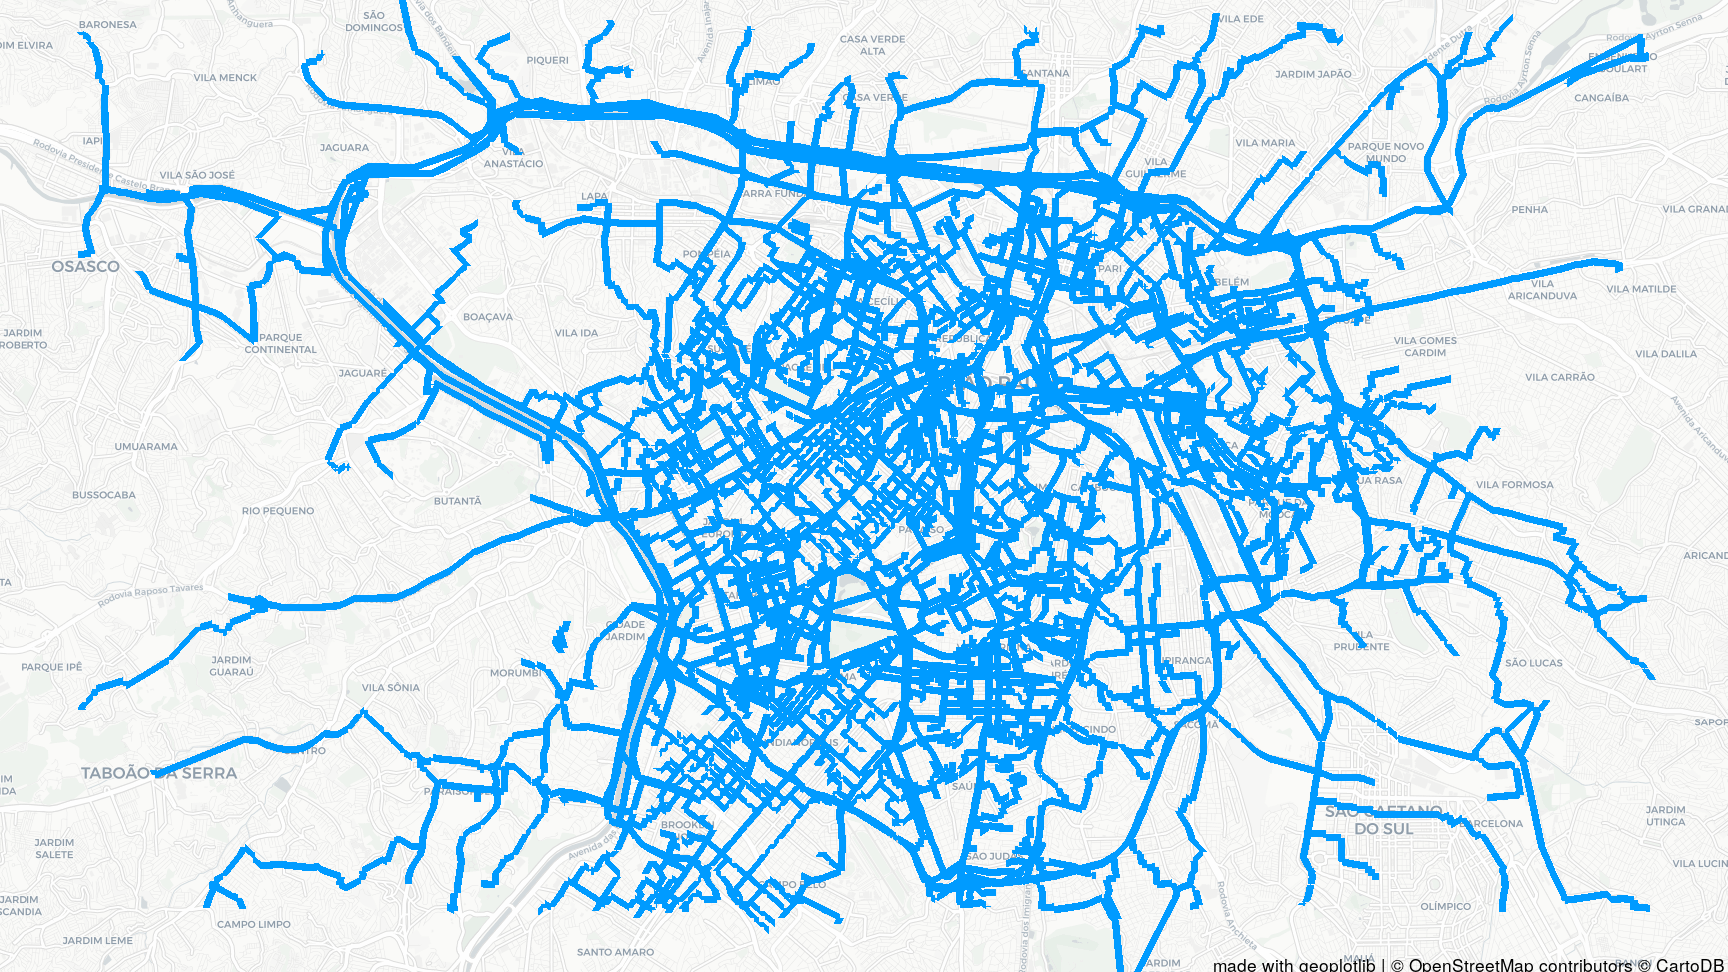
\includegraphics[width=1\textwidth]{../figuras/trafego-ocluso.png}
  \caption{Simulação do tráfego entre 6 e 7 da manhã.}
  \label{fig:simulated-traffic}
\end{figure}

\textbf{\emph{Bundling}:} para os problemas da visualização apresentados
anteriormente criaremos uma abstração com o uso do \emph{bundling} para agregar
trajetórias com origem-destino e direção similares. Utilizaremos o algoritmo
ADEB, apresentado na Seção \ref{sec:modelos-de-bundling} para aglomerar as
trajetórias em pontos de maior densidade. Com isso podemos ter uma perspectiva
dos fluxos de veículos que saem e chegam de cada região da cidade. As áreas de
maior densidade, por sua vez, informam uma quantidade maior de veículos na
região em um dado instante. Na escala da cidade, as linhas dos \emph{bundles}
podem demonstrar viagens de longa distância ou desvios realizados por alguns
veículos, sugerindo melhorias no projeto da rede rodoviária.

\textbf{\emph{Bundling} Multinível:} a dimensão espacial dos dados é o nosso
segundo parâmetro multi escala dentro da visualização. Para observar os padrões
de OD em diferentes níveis de detalhe espaciais faremos agrupamentos baseados
na escala da visualização, que está relacionada ao tamanho da área do mapa
mostrada na imagem. Este mecanismo é comumente visto em visualizações
interativas que permitem aos usuários mudar as configurações de zoom no mapa. A
partir daí, propomos um conceito de sub-trajetória, que são as partes de uma
trajetória dentro de uma sub área do mapa após um aumento do zoom.  Desta forma
detectamos os pontos dentro do escopo da sub área do mapa que formam um
subconjunto das trajetórias originais, cujas direções, origens e destinos se
tornam relativos em relação ao novo escopo. Em seguida reaplicamos o
\emph{bundling} no subconjunto. Quanto menor a escala, mais detalhes sobre o
tráfego são obtidos, sendo possível observar bairros, quadras ou até mesmo
ruas. A Figura \ref{fig:multi-scale} ilustra os diferentes níveis de detalhe
atingidos em escalas diferentes na visualização de um mapa.

\begin{figure}[!htb]
  \centering
  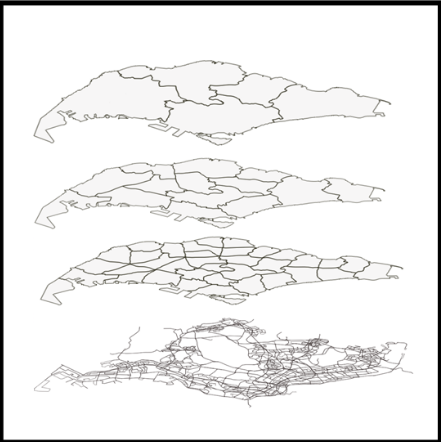
\includegraphics[width=55mm]{../figuras/multi-scale.png}
  \caption[Visualização de um mapa em diferentes escalas espaciais]{Visualização de um mapa em diferentes escalas espaciais. Fonte: \citet{Zeng2013}}
  \label{fig:multi-scale}
\end{figure}

\textbf{Parâmetros:} O algoritmo ADEB possui parâmetros que influenciam no grau
de aglomeração do \emph{bundling} e velocidade do cálculo, como por exemplo,
tamanho dos núcleos da função de densidade e tamanho da amostragem dos dados a
serem utilizadas no processo. Esses parâmetros são discutidos pelos autores do
método, e valores padrão são indicados por eles. Seguiremos inicialmente os
valores indicados, mas atentos a detalhes ou modificações que se mostrarem
necessárias. Outro parâmetro importante em nossa visualização é a escala
espacial para variação do nível de detalhes do \emph{bundling}. Esse parâmetro
age como um filtro para selecionarmos um subconjunto das trajetórias dentro de
uma sub área visualizada. Exploraremos esse parâmetro apresentando os
resultados e discussões sobre os diferentes resultados obtidos nos múltiplos
níveis.

\subsection{Visualização dos Atributos}
Depois de calcular o \emph{bundling} das trajetórias, é necessário projetar uma
maneira de mostrar a estrutura dos elementos e seus atributos. Visualizar uma
grande quantidade de atributos é ainda um desafio dentro do campo da
visualização da informação. Em nosso estudo dos fluxos de OD consideramos dois
atributos chave, densidade e fluxo, os quais destacamos diretamente na
visualização. Reconhecemos que no tráfego existem ainda outras informações
relevantes, como velocidade, aceleração, informações de gênero sobre
motoristas, mas que estas não estão no escopo desta pesquisa e devem ser
consideradas em estudos aprofundados no futuro.

\textbf{Densidade}: a densidade é uma informação importante na análise
do fluxo. Essa informação permite visualizar a quantidade de veículos se
locomovendo de uma região para outra. Esse atributo é comumente destacado de
duas formas principais, uma escala de cores, como um mapa de calor, ou através
da espessura da linha. Escolhemos escalar a espessura da linha dos
\emph{bundles} proporcionalmente à densidade do fluxo que ele representa.
Deixamos a coloração para demonstrar a direção das trajetórias, já que é uma
forma mais intuitiva para esse atributo.

\textbf{Direção}: como em \citet{Anita2017}, iremos destacar a direção das
trajetórias com um mapa de cores que indica se a trajetória está chegando ou
saindo de um ponto no mapa. É necessário ainda um cuidado com a sobreposição de
trajetórias paralelas que vão em direções opostas. \citet{Anita2017} resolvem
esse problema criando um parâmetro de repulsão para deslocar as trajetórias na
visualização, deixando mais clara a sua diferenciação.

\subsection{Visualização Interativa}

Mecanismos de interação são um excelente recurso em uma visualização de dados.
Mais do que apenas informar, os usuários podem buscar seus próprios padrões e
explorar o conteúdo à sua maneira. Adicionaremos alguns meios de interação para
facilitar o estudo das trajetórias e exploração das suas propriedades.

\textbf{Parâmetros:} Todos os parâmetros mencionados anteriormente para a exploração
multinível no tempo e no espaço serão configuráveis para os usuários da visualização,
bem como os parâmetros do algoritmo de \emph{bundling}. Desta maneira ganha-se
a liberdade para seleção dos parâmetros que melhor se adequam aos objetivos
da visualização.

\textbf{Inspecionando os \emph{bundles}}: analisando-se um \emph{bundle},
podemos dar ainda mais detalhes sobre as trajetórias que o formam para
responder duas questões importantes para análise dos fluxos: 'Qual o percentual
das trajetórias veem de uma determinada região?' ou 'Qual região é maior
responsável pelo fluxo naquele trecho?'.  Essa informação pode ser obtida
observando-se a composição do \emph{bundle} e oferece mais detalhes para que
gestores da cidade entendam melhor a estrutura do trânsito e as relações de OD.

 Para inserir esse dado na visualização recorremos a uma nova
imagem, disparada pela interação do usuário que poderá inspecionar um
\emph{bundle} para visualizar esses detalhes em uma caixa de diálogo com as
estatísticas percentuais sobre as origens das trajetórias.

\section{Visualização de Eventos Atípicos}

  Outra importante tarefa na análise do trânsito é o estudo de como a
ocorrência de eventos atípicos impactam no tráfego. Para essa tarefa, propomos
a utilização de dados que representem diferentes cenários do trânsito para
explorar como a visualização proposta ajuda na identificação desses eventos
atípicos no trânsito e como eles afetam o tráfego. Para isso, faremos uma
simulação com o InterSCSimulator e bloquearemos vias importantes da cidade por
onde passam uma grande quantidade de veículos de diversas regiões, como por
exemplo a Avenida Paulista. Esperamos que o \emph{bundling} revele as alterações nos
padrões de deslocamento dos veículos e que esses sejam visualmente
perceptíveis. Avaliar esse tipo de cenário é importante para demonstrar como a
técnica pode ajudar em questões do dia a dia no trânsito, como a ocorrência de
acidentes, alagamentos e mudanças na rede rodoviária da cidade.

\section{Avaliação da Visualização}
  Nós avaliaremos a visualização de dois pontos de vista, um qualitativo e um
quantitativo. Do ponto de vista qualitativo apontaremos o que foi alcançado com
a visualização em relação os objetivos da pesquisa de utilizar técnicas de \emph{bundling}
para visualização dos fluxos de OD no tráfego. Avaliaremos então se a visualização
tornou possível a visualização dos fluxos de OD nos diferentes níveis de
detalhe e quais foram suas limitações. Além disso, analisaremos também o potencial da
visualização com \emph{bundling} em representar mudanças no trânsito na
ocorrência de eventos atípicos, tais como o fechamento de uma rua importante do
tráfego. Dentre essas avaliações, serão experimentados os diferentes parâmetros
do algoritmo de \emph{bundling} e das técnicas de visualização utilizadas, com
uma caracterização sobre quais valores dos parâmetros foram considerados mais adequados.

  Do ponto de vista quantitativo pretendemos avaliar a escalabilidade da
solução dado o tempo de processamento para gerar a visualização de um certo
conjunto de dados. Para isso, iremos contar o tempo para gerar a visualização
ignorando etapas de pré-processamento e carregamento dos dados.

